% Options for packages loaded elsewhere
\PassOptionsToPackage{unicode}{hyperref}
\PassOptionsToPackage{hyphens}{url}
%
\documentclass[
]{article}
\usepackage{amsmath,amssymb}
\usepackage{iftex}
\ifPDFTeX
  \usepackage[T1]{fontenc}
  \usepackage[utf8]{inputenc}
  \usepackage{textcomp} % provide euro and other symbols
\else % if luatex or xetex
  \usepackage{unicode-math} % this also loads fontspec
  \defaultfontfeatures{Scale=MatchLowercase}
  \defaultfontfeatures[\rmfamily]{Ligatures=TeX,Scale=1}
\fi
\usepackage{lmodern}
\ifPDFTeX\else
  % xetex/luatex font selection
\fi
% Use upquote if available, for straight quotes in verbatim environments
\IfFileExists{upquote.sty}{\usepackage{upquote}}{}
\IfFileExists{microtype.sty}{% use microtype if available
  \usepackage[]{microtype}
  \UseMicrotypeSet[protrusion]{basicmath} % disable protrusion for tt fonts
}{}
\makeatletter
\@ifundefined{KOMAClassName}{% if non-KOMA class
  \IfFileExists{parskip.sty}{%
    \usepackage{parskip}
  }{% else
    \setlength{\parindent}{0pt}
    \setlength{\parskip}{6pt plus 2pt minus 1pt}}
}{% if KOMA class
  \KOMAoptions{parskip=half}}
\makeatother
\usepackage{xcolor}
\usepackage[margin=1in]{geometry}
\usepackage{color}
\usepackage{fancyvrb}
\newcommand{\VerbBar}{|}
\newcommand{\VERB}{\Verb[commandchars=\\\{\}]}
\DefineVerbatimEnvironment{Highlighting}{Verbatim}{commandchars=\\\{\}}
% Add ',fontsize=\small' for more characters per line
\usepackage{framed}
\definecolor{shadecolor}{RGB}{248,248,248}
\newenvironment{Shaded}{\begin{snugshade}}{\end{snugshade}}
\newcommand{\AlertTok}[1]{\textcolor[rgb]{0.94,0.16,0.16}{#1}}
\newcommand{\AnnotationTok}[1]{\textcolor[rgb]{0.56,0.35,0.01}{\textbf{\textit{#1}}}}
\newcommand{\AttributeTok}[1]{\textcolor[rgb]{0.13,0.29,0.53}{#1}}
\newcommand{\BaseNTok}[1]{\textcolor[rgb]{0.00,0.00,0.81}{#1}}
\newcommand{\BuiltInTok}[1]{#1}
\newcommand{\CharTok}[1]{\textcolor[rgb]{0.31,0.60,0.02}{#1}}
\newcommand{\CommentTok}[1]{\textcolor[rgb]{0.56,0.35,0.01}{\textit{#1}}}
\newcommand{\CommentVarTok}[1]{\textcolor[rgb]{0.56,0.35,0.01}{\textbf{\textit{#1}}}}
\newcommand{\ConstantTok}[1]{\textcolor[rgb]{0.56,0.35,0.01}{#1}}
\newcommand{\ControlFlowTok}[1]{\textcolor[rgb]{0.13,0.29,0.53}{\textbf{#1}}}
\newcommand{\DataTypeTok}[1]{\textcolor[rgb]{0.13,0.29,0.53}{#1}}
\newcommand{\DecValTok}[1]{\textcolor[rgb]{0.00,0.00,0.81}{#1}}
\newcommand{\DocumentationTok}[1]{\textcolor[rgb]{0.56,0.35,0.01}{\textbf{\textit{#1}}}}
\newcommand{\ErrorTok}[1]{\textcolor[rgb]{0.64,0.00,0.00}{\textbf{#1}}}
\newcommand{\ExtensionTok}[1]{#1}
\newcommand{\FloatTok}[1]{\textcolor[rgb]{0.00,0.00,0.81}{#1}}
\newcommand{\FunctionTok}[1]{\textcolor[rgb]{0.13,0.29,0.53}{\textbf{#1}}}
\newcommand{\ImportTok}[1]{#1}
\newcommand{\InformationTok}[1]{\textcolor[rgb]{0.56,0.35,0.01}{\textbf{\textit{#1}}}}
\newcommand{\KeywordTok}[1]{\textcolor[rgb]{0.13,0.29,0.53}{\textbf{#1}}}
\newcommand{\NormalTok}[1]{#1}
\newcommand{\OperatorTok}[1]{\textcolor[rgb]{0.81,0.36,0.00}{\textbf{#1}}}
\newcommand{\OtherTok}[1]{\textcolor[rgb]{0.56,0.35,0.01}{#1}}
\newcommand{\PreprocessorTok}[1]{\textcolor[rgb]{0.56,0.35,0.01}{\textit{#1}}}
\newcommand{\RegionMarkerTok}[1]{#1}
\newcommand{\SpecialCharTok}[1]{\textcolor[rgb]{0.81,0.36,0.00}{\textbf{#1}}}
\newcommand{\SpecialStringTok}[1]{\textcolor[rgb]{0.31,0.60,0.02}{#1}}
\newcommand{\StringTok}[1]{\textcolor[rgb]{0.31,0.60,0.02}{#1}}
\newcommand{\VariableTok}[1]{\textcolor[rgb]{0.00,0.00,0.00}{#1}}
\newcommand{\VerbatimStringTok}[1]{\textcolor[rgb]{0.31,0.60,0.02}{#1}}
\newcommand{\WarningTok}[1]{\textcolor[rgb]{0.56,0.35,0.01}{\textbf{\textit{#1}}}}
\usepackage{graphicx}
\makeatletter
\def\maxwidth{\ifdim\Gin@nat@width>\linewidth\linewidth\else\Gin@nat@width\fi}
\def\maxheight{\ifdim\Gin@nat@height>\textheight\textheight\else\Gin@nat@height\fi}
\makeatother
% Scale images if necessary, so that they will not overflow the page
% margins by default, and it is still possible to overwrite the defaults
% using explicit options in \includegraphics[width, height, ...]{}
\setkeys{Gin}{width=\maxwidth,height=\maxheight,keepaspectratio}
% Set default figure placement to htbp
\makeatletter
\def\fps@figure{htbp}
\makeatother
\setlength{\emergencystretch}{3em} % prevent overfull lines
\providecommand{\tightlist}{%
  \setlength{\itemsep}{0pt}\setlength{\parskip}{0pt}}
\setcounter{secnumdepth}{-\maxdimen} % remove section numbering
\ifLuaTeX
  \usepackage{selnolig}  % disable illegal ligatures
\fi
\usepackage{bookmark}
\IfFileExists{xurl.sty}{\usepackage{xurl}}{} % add URL line breaks if available
\urlstyle{same}
\hypersetup{
  pdftitle={CodingChallenge5},
  pdfauthor={Kylie Blake},
  hidelinks,
  pdfcreator={LaTeX via pandoc}}

\title{CodingChallenge5}
\author{Kylie Blake}
\date{2025-03-22}

\begin{document}
\maketitle

{
\setcounter{tocdepth}{2}
\tableofcontents
}
\section{Question 1}\label{question-1}

\textbf{1. 3 pts. Download two .csv files from Canvas called
DiversityData.csv and Metadata.csv, and read them into R using relative
file paths.}

\begin{Shaded}
\begin{Highlighting}[]
\CommentTok{\#Loading in necessary packages}
\FunctionTok{library}\NormalTok{(tidyverse)}
\end{Highlighting}
\end{Shaded}

\begin{verbatim}
## -- Attaching core tidyverse packages ------------------------ tidyverse 2.0.0 --
## v dplyr     1.1.4     v readr     2.1.5
## v forcats   1.0.0     v stringr   1.5.1
## v ggplot2   3.5.1     v tibble    3.2.1
## v lubridate 1.9.4     v tidyr     1.3.1
## v purrr     1.0.2     
## -- Conflicts ------------------------------------------ tidyverse_conflicts() --
## x dplyr::filter() masks stats::filter()
## x dplyr::lag()    masks stats::lag()
## i Use the conflicted package (<http://conflicted.r-lib.org/>) to force all conflicts to become errors
\end{verbatim}

\begin{Shaded}
\begin{Highlighting}[]
\FunctionTok{library}\NormalTok{(ggplot2)}

\CommentTok{\#Loading in DiversityData and Metadata}
\NormalTok{Metadata }\OtherTok{\textless{}{-}} \FunctionTok{read.csv}\NormalTok{(}\StringTok{"CodingChallenge5//Metadata.csv"}\NormalTok{, }\AttributeTok{na.strings =} \StringTok{"na"}\NormalTok{)}
\NormalTok{DiversityData }\OtherTok{\textless{}{-}}  \FunctionTok{read.csv}\NormalTok{(}\StringTok{"CodingChallenge5//DiversityData.csv"}\NormalTok{)}
\end{Highlighting}
\end{Shaded}

\section{Question 2}\label{question-2}

\textbf{2. 4 pts. Join the two dataframes together by the common column
`Code'. Name the resulting dataframe alpha.}

\begin{Shaded}
\begin{Highlighting}[]
\CommentTok{\#Combining the two datasets by column "Code"}
\NormalTok{alpha }\OtherTok{\textless{}{-}} \FunctionTok{left\_join}\NormalTok{(Metadata,DiversityData, }\AttributeTok{by =} \StringTok{"Code"}\NormalTok{)}
\FunctionTok{head}\NormalTok{(alpha) }\CommentTok{\#viewing first few rows of dataframe}
\end{Highlighting}
\end{Shaded}

\begin{verbatim}
##     Code Crop Time_Point Replicate Water_Imbibed  shannon invsimpson   simpson
## 1 S01_13 Soil          0         1            NA 6.624921   210.7279 0.9952545
## 2 S02_16 Soil          0         2            NA 6.612413   206.8666 0.9951660
## 3 S03_19 Soil          0         3            NA 6.660853   213.0184 0.9953056
## 4 S04_22 Soil          0         4            NA 6.660671   204.6908 0.9951146
## 5 S05_25 Soil          0         5            NA 6.610965   200.2552 0.9950064
## 6 S06_28 Soil          0         6            NA 6.650812   199.3211 0.9949830
##   richness
## 1     3319
## 2     3079
## 3     3935
## 4     3922
## 5     3196
## 6     3481
\end{verbatim}

\section{Question 3}\label{question-3}

\textbf{3. 4 pts. Calculate Pielou's evenness index: Pielou's evenness
is an ecological parameter calculated by the Shannon diversity index
(column Shannon) divided by the log of the richness column.} \textbf{a.
Using mutate, create a new column to calculate Pielou's evenness index.}
\textbf{b. Name the resulting dataframe alpha\_even.}

\begin{Shaded}
\begin{Highlighting}[]
\CommentTok{\#Creating Pielous\textquotesingle{}s evenness index column, named PEI}
\NormalTok{alpha\_even }\OtherTok{\textless{}{-}} \FunctionTok{mutate}\NormalTok{(alpha, }\AttributeTok{PEI =}\NormalTok{ shannon}\SpecialCharTok{/}\FunctionTok{log}\NormalTok{(richness))}
\FunctionTok{head}\NormalTok{(alpha\_even) }\CommentTok{\#viewing first few rows of dataframe}
\end{Highlighting}
\end{Shaded}

\begin{verbatim}
##     Code Crop Time_Point Replicate Water_Imbibed  shannon invsimpson   simpson
## 1 S01_13 Soil          0         1            NA 6.624921   210.7279 0.9952545
## 2 S02_16 Soil          0         2            NA 6.612413   206.8666 0.9951660
## 3 S03_19 Soil          0         3            NA 6.660853   213.0184 0.9953056
## 4 S04_22 Soil          0         4            NA 6.660671   204.6908 0.9951146
## 5 S05_25 Soil          0         5            NA 6.610965   200.2552 0.9950064
## 6 S06_28 Soil          0         6            NA 6.650812   199.3211 0.9949830
##   richness       PEI
## 1     3319 0.8171431
## 2     3079 0.8232216
## 3     3935 0.8046776
## 4     3922 0.8049774
## 5     3196 0.8192376
## 6     3481 0.8155427
\end{verbatim}

\section{Question 4}\label{question-4}

\textbf{4. 4. Pts. Using tidyverse language of functions and the pipe,
use the summarise function and tell me the mean and standard error
evenness grouped by crop over time.} \textbf{a. Start with the
alpha\_even dataframe} \textbf{b. Group the data: group the data by Crop
and Time\_Point.} \textbf{c.~Summarize the data: Calculate the mean,
count, standard deviation, and standard error for the even variable
within each group.}

\begin{Shaded}
\begin{Highlighting}[]
\CommentTok{\#caluculate summary statistics for evenness grouped by crop over time}
\NormalTok{alpha\_average }\OtherTok{\textless{}{-}}\NormalTok{  alpha\_even }\SpecialCharTok{\%\textgreater{}\%} 
  \FunctionTok{group\_by}\NormalTok{(Crop, Time\_Point) }\SpecialCharTok{\%\textgreater{}\%} \CommentTok{\#viewing data grouped by crop and time\_point}
  \FunctionTok{summarise}\NormalTok{(}\AttributeTok{mean.even =} \FunctionTok{mean}\NormalTok{(PEI), }\CommentTok{\#calculate mean evenness}
            \AttributeTok{count =} \FunctionTok{n}\NormalTok{(), }\CommentTok{\#count number of values by crop over time}
            \AttributeTok{sd.even =} \FunctionTok{sd}\NormalTok{(PEI), }\CommentTok{\#calculate std dev evenness}
            \AttributeTok{se.even =}\NormalTok{ sd.even}\SpecialCharTok{/}\FunctionTok{sqrt}\NormalTok{(count)) }\CommentTok{\#calculate std error evenness}
\end{Highlighting}
\end{Shaded}

\begin{verbatim}
## `summarise()` has grouped output by 'Crop'. You can override using the
## `.groups` argument.
\end{verbatim}

\begin{Shaded}
\begin{Highlighting}[]
\FunctionTok{head}\NormalTok{(alpha\_average) }\CommentTok{\#view some of the resulting alpha\_average dataframe}
\end{Highlighting}
\end{Shaded}

\begin{verbatim}
## # A tibble: 6 x 6
## # Groups:   Crop [2]
##   Crop   Time_Point mean.even count sd.even se.even
##   <chr>       <int>     <dbl> <int>   <dbl>   <dbl>
## 1 Cotton          0     0.820     6 0.00556 0.00227
## 2 Cotton          6     0.805     6 0.00920 0.00376
## 3 Cotton         12     0.767     6 0.0157  0.00640
## 4 Cotton         18     0.755     5 0.0169  0.00755
## 5 Soil            0     0.814     6 0.00765 0.00312
## 6 Soil            6     0.810     6 0.00587 0.00240
\end{verbatim}

\section{Question 5}\label{question-5}

\textbf{5. 4. Pts. Calculate the difference between the soybean column,
the soil column, and the difference between the cotton column and the
soil column} \textbf{a. Start with the alpha\_average dataframe}
\textbf{b. Select relevant columns: select the columns Time\_Point,
Crop, and mean.even.} \textbf{c.~Reshape the data: Use the pivot\_wider
function to transform the data from long to wide format, creating new
columns for each Crop with values from mean.even.} \textbf{d.~Calculate
differences: Create new columns named diff.cotton.even and
diff.soybean.even by calculating the difference between Soil and Cotton,
and Soil and Soybean, respectively.} \textbf{e. Name the resulting
dataframe alpha\_average2}

\begin{Shaded}
\begin{Highlighting}[]
\NormalTok{alpha\_average2 }\OtherTok{\textless{}{-}}\NormalTok{ alpha\_average }\SpecialCharTok{\%\textgreater{}\%} 
  \FunctionTok{select}\NormalTok{(Time\_Point, Crop, mean.even) }\SpecialCharTok{\%\textgreater{}\%} \CommentTok{\#only select the three columns (Time\_Point, Crop, mean.even)}
  \FunctionTok{pivot\_wider}\NormalTok{(}\AttributeTok{names\_from =}\NormalTok{ Crop, }\AttributeTok{values\_from =}\NormalTok{ mean.even) }\SpecialCharTok{\%\textgreater{}\%}  \CommentTok{\#put multiple observations in one row for separate columns by Crop}
  \FunctionTok{mutate}\NormalTok{(}\AttributeTok{diff.cotton.even =}\NormalTok{ Soil }\SpecialCharTok{{-}}\NormalTok{ Cotton,}
         \AttributeTok{diff.soybean.even =}\NormalTok{ Soil }\SpecialCharTok{{-}}\NormalTok{ Soybean) }\CommentTok{\#create new columns }
\FunctionTok{head}\NormalTok{(alpha\_average2) }\CommentTok{\#view some of the resulting alpha\_average2 dataframe}
\end{Highlighting}
\end{Shaded}

\begin{verbatim}
## # A tibble: 4 x 6
##   Time_Point Cotton  Soil Soybean diff.cotton.even diff.soybean.even
##        <int>  <dbl> <dbl>   <dbl>            <dbl>             <dbl>
## 1          0  0.820 0.814   0.822         -0.00602          -0.00740
## 2          6  0.805 0.810   0.764          0.00507           0.0459 
## 3         12  0.767 0.798   0.687          0.0313            0.112  
## 4         18  0.755 0.800   0.716          0.0449            0.0833
\end{verbatim}

\section{Question 6}\label{question-6}

\textbf{6. 4 pts. Connecting it to plots} \textbf{a. Start with the
alpha\_average2 dataframe} \textbf{b. Select relevant columns: select
the columns Time\_Point, diff.cotton.even, and diff.soybean.even.}
\textbf{c.~Reshape the data: Use the pivot\_longer function to transform
the data from wide to long format, creating a new column named diff that
contains the values from diff.cotton.even and diff.soybean.even.}
\textbf{i. This might be challenging, so I'll give you a break. The code
is below.} \textbf{d.~Create the plot: Use ggplot and geom\_line() with
`Time\_Point' on the x-axis, the column `values' on the y-axis, and
different colors for each `diff' category. The column named `values'
come from the pivot\_longer. The resulting plot should look like the one
to the right.}

\begin{Shaded}
\begin{Highlighting}[]
\NormalTok{alpha\_average2 }\SpecialCharTok{\%\textgreater{}\%} 
  \FunctionTok{select}\NormalTok{(Time\_Point, diff.cotton.even,diff.soybean.even) }\SpecialCharTok{\%\textgreater{}\%}\CommentTok{\#selecting only relevant columns}
  \FunctionTok{pivot\_longer}\NormalTok{(}\FunctionTok{c}\NormalTok{(diff.cotton.even, diff.soybean.even), }\AttributeTok{names\_to =} \StringTok{"diff"}\NormalTok{) }\SpecialCharTok{\%\textgreater{}\%} \CommentTok{\#putting data in long format }
  \FunctionTok{ggplot}\NormalTok{(}\FunctionTok{aes}\NormalTok{(}\AttributeTok{x =}\NormalTok{ Time\_Point, }\AttributeTok{y =}\NormalTok{ value, }\AttributeTok{color =}\NormalTok{ diff)) }\SpecialCharTok{+} \CommentTok{\# adding in a ggplot}
  \FunctionTok{geom\_line}\NormalTok{() }\SpecialCharTok{+} \CommentTok{\#make line bar}
  \FunctionTok{xlab}\NormalTok{(}\StringTok{"Time (hrs)"}\NormalTok{) }\SpecialCharTok{+} \CommentTok{\#label x{-}axis}
  \FunctionTok{ylab}\NormalTok{(}\StringTok{"difference from soil in Pielou\textquotesingle{}s evenness"}\NormalTok{) }\CommentTok{\#label y{-}axis}
\end{Highlighting}
\end{Shaded}

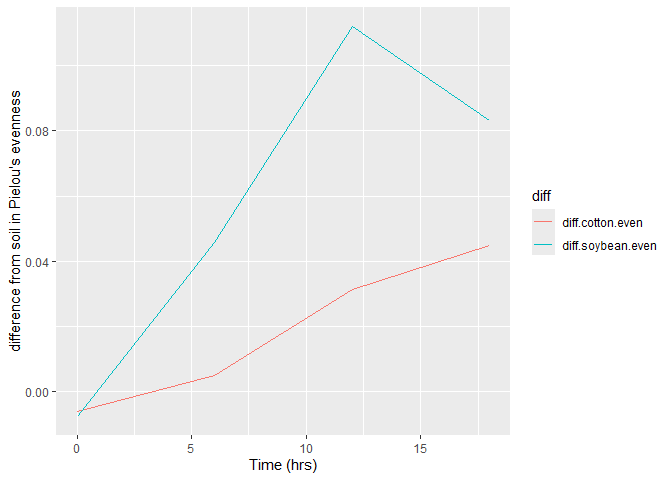
\includegraphics{Blake_CodingChallenge5_files/figure-latex/unnamed-chunk-6-1.pdf}

\section{Question 7}\label{question-7}

\begin{enumerate}
\def\labelenumi{\arabic{enumi}.}
\setcounter{enumi}{6}
\tightlist
\item
  2 pts. Commit and push a gfm .md file to GitHub inside a directory
  called Coding Challenge 5. Provide me a link to your github written as
  a clickable link in your .pdf or .docx
\end{enumerate}

\textbf{\href{https://github.com/kzb0180}{Click here to my GitHub}}

\end{document}
